%%%%%%%%%%%%%%%%%%%%%%%%%%%%%%%%%%%%%%%%%%%%%%%
\chapter{Further Simulations to Support the Rayleigh Channel} \label{chap:Experiments}
%%%%%%%%%%%%%%%%%%%%%%%%%%%%%%%%%%%%%%%%%%%%%%%
\graphicspath{{C:/Users/Kevin/Bachelarbeit/Bachelorarbeit/01_Bachelorarbeit_LaTex/02_Figures/}}

In this chapter we will discuss further simulations done to support the previous chapters. First of all a simulation to compare the \gls{FER} simulated in chapter 5 will be initialized.
\section{Simulated Rayleigh FER with AWGN Channel}
\label{RAYAWGN}

In this section a simulation based on the AWGN channel will be done to create a theoretical \gls{FER} for a Rayleigh channel. This is done to have a reliable comparison for our simulation in Chapter 5. 
With the AWGN channel the reliability of the channel has already been proven with the capacity calculations from chapter 3. In chapter 4 the \gls{FER} from the AWGN channel was in range of 0\,dB up to 5\,dB SNR. In this region a valid \gls{FER} was given with the number of frames set. 
For this simulation first of all an AWGN channel will be simulated for the given range of 0\,dB to 5\,dB SNR. Then SNR from 0\,dB to 50\,dB SNR will be initialized. The SNR will be modulated with complex Gaussian noise to simulate the Rayleigh fading channel. For the now modulated SNR the corresponding \gls{FER} can now be picked out. To get reliable results the \gls{MC} will be applied again. For every step of SNR many independent fading coefficients will be created. The mean of all \gls{FER} values will be taken to get the final data point plotted for the corresponding \gls{SNR} value.    

\begin{equation}
SNR_{ray} = SNR_{AWGN} * \textbf{H}
\end{equation}
\begin{equation}
FER_{ray} = FER_{AWGN}(SNR_{ray})
\end{equation}

\begin{figure}[!htb]
	\setlength\fwidth{0.8\textwidth}
	\setlength\fheight{0.4\textheight}
    \centering
    % This file was created by matlab2tikz.
%
%The latest updates can be retrieved from
%  http://www.mathworks.com/matlabcentral/fileexchange/22022-matlab2tikz-matlab2tikz
%where you can also make suggestions and rate matlab2tikz.
%
\definecolor{mycolor1}{rgb}{0.00000,0.44700,0.74100}%
%
\begin{tikzpicture}

\begin{axis}[%
width=0.951\fwidth,
height=\fheight,
at={(0\fwidth,0\fheight)},
scale only axis,
xmin=0,
xmax=6,
xlabel style={font=\color{white!15!black}},
xlabel={SNR in dB},
ymode=log,
ymin=1e-10,
ymax=1,
yminorticks=true,
ylabel style={font=\color{white!15!black}},
ylabel={FER},
axis background/.style={fill=white},
title style={font=\bfseries},
title={FER in AWGN Channel},
xmajorgrids,
ymajorgrids,
yminorgrids,
legend style={legend cell align=left, align=left, draw=white!15!black}
]
\addplot [color=mycolor1, line width=1.0pt]
  table[row sep=crcr]{%
0	0.970873786407765\\
1	0.561801025423803\\
2	0.0274983941638387\\
3	0.000110109540972448\\
4	2.20000440021017e-10\\
};

\end{axis}
\end{tikzpicture}%
    \caption{FER for a simulated AWGN channel}
    \label{fig:FERAWGN}
\end{figure}
In \fig{fig:FERAWGN} the \gls{FER} for the AWGN channel is depicted. As mentioned above the valid range is only for 0\,dB up to 5\,dB, which will be a problem for higher \gls{SNR} values. For higher SNR values an error floor must be initialized. The error floor is the lowest probability the \gls{FER} can take. It is proven that every transmission will have a small probability of failure, no transmission will have 0 \gls{FER} which would mean that a transmission can always be without any errors. In practical transmissions this is not achievable.

\begin{figure}[!h]
	\setlength\fwidth{0.9\textwidth}
	\setlength\fheight{0.4\textheight}
	\centering
	% This file was created by matlab2tikz.
%
%The latest updates can be retrieved from
%  http://www.mathworks.com/matlabcentral/fileexchange/22022-matlab2tikz-matlab2tikz
%where you can also make suggestions and rate matlab2tikz.
%
\definecolor{mycolor1}{rgb}{0.00000,0.44700,0.74100}%
%
\begin{tikzpicture}

\begin{axis}
[%
width=0.951\fwidth,
height=\fheight,
at={(0\fwidth,0\fheight)},
scale only axis,
xmin=0,
xmax=50,
xlabel style={font=\color{white!15!black}},
xlabel={SNR in dB},
ymode=log,
ymin=1e-10,
ymax=1,
yminorticks=true,
ylabel style={font=\color{white!15!black}},
ylabel={FER},
axis background/.style={fill=white},
title style={font=\bfseries},
title={Rayleigh FER based on AWGN channel},
xmajorgrids,
ymajorgrids,
yminorgrids,
legend style={at={(0.9,0.3)}, legend cell align=left, align=left, draw=white!15!black}
]
\addplot [color=red, line width=1.5pt]
  table[row sep=crcr]{%
1	0.0830532513909396\\
2	0.0820282360688762\\
3	0.0754327795430033\\
5	0.0603613555110878\\
6	0.0509930163048139\\
7	0.0422618648071782\\
8	0.0359539585157046\\
9	0.0294870809109138\\
10	0.0245515499744151\\
12	0.0158080363301829\\
13	0.0131127925120529\\
14	0.010460998386777\\
15	0.00817327921756875\\
16	0.00644695372104698\\
17	0.00531896244094089\\
18	0.00454545734103555\\
19	0.00363205436224636\\
20	0.00262877600942798\\
21	0.00200270126361543\\
22	0.00177094037964383\\
23	0.00144694437921257\\
24	0.00107998833890822\\
25	0.000868778722335362\\
26	0.000748991111319098\\
27	0.00052671472774556\\
28	0.000412561625682911\\
29	0.000355199585321207\\
30	0.000225346995078924\\
31	0.000168101367597243\\
32	0.000208718351011472\\
33	0.000143591355222299\\
34	0.00010413121202644\\
35	8.96476319060739e-05\\
36	0.000101692393633131\\
37	4.68147789693424e-05\\
38	4.70123362336143e-05\\
39	2.64485894283113e-05\\
40	3.128923952961e-05\\
41	2.05428037427835e-05\\
42	1.91421453042016e-05\\
43	1.51385247710512e-05\\
44	1.38924684715064e-05\\
45	5.58377839712014e-06\\
46	2.07824582232808e-05\\
47	4.07076470136795e-07\\
48	4.79031328066027e-06\\
49	2.78639032195876e-06\\
50	1.10235102351024e-10\\
};
\addlegendentry{Estimated Rayleigh FER, ErrorFloor: 0}

\addplot [color=green, line width=1.5pt]
  table[row sep=crcr]{%
1	0.588273382855458\\
3	0.433631634923674\\
4	0.357531315427569\\
5	0.29908565890299\\
7	0.201162965267364\\
8	0.164359300046626\\
9	0.129549643741209\\
10	0.107073987923644\\
12	0.0672833333235462\\
13	0.0547966317588708\\
15	0.0346155857147029\\
16	0.0286550031056596\\
17	0.0222321743519897\\
18	0.0177828158472179\\
19	0.0144900880658035\\
20	0.0104018698422347\\
21	0.00930286224016606\\
22	0.0072179587879032\\
23	0.00549372375872881\\
25	0.00366952045085021\\
26	0.00271413725076233\\
27	0.00231897059529153\\
28	0.00174871976919339\\
29	0.00152637776888243\\
31	0.000896873652706296\\
32	0.000905136714188982\\
33	0.000636354037085892\\
34	0.000455704210982692\\
35	0.00031693663529356\\
36	0.00041397555399065\\
37	0.000156425943507997\\
38	0.000219150700566799\\
40	0.000103221060453958\\
41	5.18480701625414e-05\\
42	7.86068192770881e-05\\
43	4.11678927704388e-05\\
44	2.10735195891598e-05\\
45	4.0318698695939e-05\\
46	1.48435948403267e-05\\
47	3.11551319812111e-05\\
48	4.12329547271343e-05\\
49	1.00000000000018e-06\\
50	1.00000000000018e-06\\
};
\addlegendentry{$\text{Estimated Rayleigh FER, ErrorFloor: 10}^\text{-6}$}

\addplot [color=mycolor1, line width=1.5pt]
  table[row sep=crcr]{%
0	0.970873786407765\\
0.308910617821235	0.844505856132907\\
0.578481156962313	0.73423100920599\\
0.813821627643255	0.637958862914563\\
1.00567201134402	0.558767182602191\\
1.14677229354459	0.483376939975421\\
1.27041254082508	0.417315638782124\\
1.37888275776552	0.359359723702564\\
1.4741929483859	0.30843524443426\\
1.55807311614623	0.263617855691996\\
1.63200326400653	0.224116788098818\\
1.69726339452679	0.189248133004396\\
1.75491350982702	0.158445528557667\\
1.80585361170722	0.131228101488867\\
1.8508037016074	0.107211153182181\\
1.89033378066756	0.0860901305667569\\
1.9249138498277	0.0676139109350506\\
1.95487390974782	0.0516061740881472\\
1.98048396096792	0.0379226580451165\\
2.00771401542803	0.0272839385766701\\
2.14267428534857	0.0235880261662036\\
2.26098452196904	0.0203480780535605\\
2.36483472966946	0.0175041205563247\\
2.45612491224982	0.0150041217125822\\
2.53650507301015	0.0128028958711973\\
2.60739521479043	0.0108615559869503\\
2.66998533997068	0.00914751362053727\\
2.7252954505909	0.00763283582398344\\
2.7741455482911	0.00629506669793654\\
2.81721563443127	0.00511558427708002\\
2.85504571009142	0.00407960053013313\\
2.88803577607155	0.00317616135985089\\
2.91650583301167	0.00239650348843727\\
2.94069588139176	0.00173405445754526\\
2.96076592153184	0.00118443262827686\\
2.97684595369191	0.00074407791902744\\
2.98905597811196	0.000409704100623486\\
2.99748599497199	0.000178846501184893\\
3.00459600919202	0.000109494438988878\\
3.13944627889256	9.46609093218187e-05\\
3.25765651531303	8.16577833155666e-05\\
3.36141672283345	7.02441604883208e-05\\
3.45263690527381	6.02099404198807e-05\\
3.53295706591413	5.13747227494456e-05\\
3.60378720757442	4.35834071668143e-05\\
3.66632733265467	3.67039934079867e-05\\
3.72159744319489	3.06242812485626e-05\\
3.77041754083508	2.5254070508141e-05\\
3.81345762691525	2.05196610393221e-05\\
3.8512477024954	1.63627527255054e-05\\
3.88420776841554	1.27371454742909e-05\\
3.91265782531565	9.60763921527843e-06\\
3.93681787363575	6.9500339000678e-06\\
3.95686791373583	4.74452948905898e-06\\
3.97292794585589	2.97792595585191e-06\\
3.98510797021594	1.63812327624653e-06\\
3.99351798703597	7.13021426042853e-07\\
3.99831799663599	1.85020370040725e-07\\
3.999937999876	6.82001364001651e-09\\
3.999997999996	2.20000440021017e-10\\
};
\addlegendentry{AWGN FER}

\end{axis}
\end{tikzpicture}%
	\caption{Comparison between AWGN FER and Rayleigh FER}
	\label{fig:FERAWGNRAY}
\end{figure}
\newpage
In \fig{fig:FERAWGNRAY} the \gls{FER} of the AWGN channel is compared to the simulated \gls{FER} of the rayleigh channel with error floors of $0$ and $10^{-6}$. It can be observed that Rayleigh fading deteriorates the channel performace by a lot in comparison to the simple AWGN channel. Furthermore as seen in the graphic the value of the error floor also needs to be determined. There is a offset when simulating the \gls{FER} for different error floors, with the 0 error floor achieving way better \gls{FER} than the one with an error floor of $10^{-6}$. Comparing the now simulated theoretical Rayleigh \gls{FER} with the previously simulated Rayleigh channel in Chapter 5 a definite answer for the previously implemented Rayleigh channel can be given.
\newpage
\begin{figure}[!htb]
	\setlength\fwidth{0.95\textwidth}
	\setlength\fheight{0.4\textheight}
	\centering
	% This file was created by matlab2tikz.
%
%The latest updates can be retrieved from
%  http://www.mathworks.com/matlabcentral/fileexchange/22022-matlab2tikz-matlab2tikz
%where you can also make suggestions and rate matlab2tikz.
%
\definecolor{mycolor1}{rgb}{0.00000,0.44700,0.74100}%
\definecolor{mycolor2}{rgb}{0.49020,0.18039,0.56078}%
%
\begin{tikzpicture}

\begin{axis}[%
width=0.951\fwidth,
height=\fheight,
at={(0\fwidth,0\fheight)},
scale only axis,
xmin=0,
xmax=50,
xlabel style={font=\color{white!15!black}},
xlabel={SNR in dB},
ymode=log,
ymin=1e-10,
ymax=1,
yminorticks=true,
ylabel style={font=\color{white!15!black}},
ylabel={FER},
axis background/.style={fill=white},
title style={font=\bfseries},
title={Comparison between both Rayleigh FER},
xmajorgrids,
ymajorgrids,
yminorgrids,
legend style={at={(0.1,0.1)}, anchor=south west, legend cell align=left, align=left, draw=white!15!black}
]
\addplot [color=red, dotted, line width=1.5pt]
  table[row sep=crcr]{%
1	0.0830532513909396\\
2	0.0820282360688762\\
3	0.0754327795430033\\
5	0.0603613555110878\\
6	0.0509930163048139\\
7	0.0422618648071782\\
8	0.0359539585157046\\
9	0.0294870809109138\\
10	0.0245515499744151\\
12	0.0158080363301829\\
13	0.0131127925120529\\
14	0.010460998386777\\
15	0.00817327921756875\\
16	0.00644695372104698\\
17	0.00531896244094089\\
18	0.00454545734103555\\
19	0.00363205436224636\\
20	0.00262877600942798\\
21	0.00200270126361543\\
22	0.00177094037964383\\
23	0.00144694437921257\\
24	0.00107998833890822\\
25	0.000868778722335362\\
26	0.000748991111319098\\
27	0.00052671472774556\\
28	0.000412561625682911\\
29	0.000355199585321207\\
30	0.000225346995078924\\
31	0.000168101367597243\\
32	0.000208718351011472\\
33	0.000143591355222299\\
34	0.00010413121202644\\
35	8.96476319060739e-05\\
36	0.000101692393633131\\
37	4.68147789693424e-05\\
38	4.70123362336143e-05\\
39	2.64485894283113e-05\\
40	3.128923952961e-05\\
41	2.05428037427835e-05\\
42	1.91421453042016e-05\\
43	1.51385247710512e-05\\
44	1.38924684715064e-05\\
45	5.58377839712014e-06\\
46	2.07824582232808e-05\\
47	4.07076470136795e-07\\
48	4.79031328066027e-06\\
49	2.78639032195876e-06\\
50	1.10235102351024e-10\\
};
\addlegendentry{Estimated Rayleigh FER, ErrorFloor: 0}

\addplot [color=green, dotted, line width=1.5pt]
  table[row sep=crcr]{%
1	0.588273382855458\\
3	0.433631634923674\\
4	0.357531315427569\\
5	0.29908565890299\\
7	0.201162965267364\\
8	0.164359300046626\\
9	0.129549643741209\\
10	0.107073987923644\\
12	0.0672833333235462\\
13	0.0547966317588708\\
15	0.0346155857147029\\
16	0.0286550031056596\\
17	0.0222321743519897\\
18	0.0177828158472179\\
19	0.0144900880658035\\
20	0.0104018698422347\\
21	0.00930286224016606\\
22	0.0072179587879032\\
23	0.00549372375872881\\
25	0.00366952045085021\\
26	0.00271413725076233\\
27	0.00231897059529153\\
28	0.00174871976919339\\
29	0.00152637776888243\\
31	0.000896873652706296\\
32	0.000905136714188982\\
33	0.000636354037085892\\
34	0.000455704210982692\\
35	0.00031693663529356\\
36	0.00041397555399065\\
37	0.000156425943507997\\
38	0.000219150700566799\\
40	0.000103221060453958\\
41	5.18480701625414e-05\\
42	7.86068192770881e-05\\
43	4.11678927704388e-05\\
44	2.10735195891598e-05\\
45	4.0318698695939e-05\\
46	1.48435948403267e-05\\
47	3.11551319812111e-05\\
48	4.12329547271343e-05\\
49	1.00000000000018e-06\\
50	1.00000000000018e-06\\
};
\addlegendentry{$\text{Estimated Rayleigh FER, ErrorFloor: 10}^\text{-}^\text{6}$}

\addplot [color=red, draw=none, mark=asterisk, mark options={solid, red}]
  table[row sep=crcr]{%
20.973	0.01\\
};


\addplot [color=green, draw=none, mark=asterisk, mark options={solid, green}]
  table[row sep=crcr]{%
30.728	0.001\\
};


\addplot [color=mycolor1, line width=1.5pt]
  table[row sep=crcr]{%
0	0.735294117647055\\
0.603012060241205	0.640464781413951\\
1.05002100042001	0.579073503868051\\
2.04304086081721	0.594767233153896\\
2.86005720114402	0.518170406957404\\
3.08506170123403	0.49302157760327\\
3.53607072141443	0.429242524244421\\
3.92907858157163	0.373665655131284\\
4.02508050161003	0.363537944401793\\
5.04510090201804	0.356338144000369\\
5.65911318226365	0.310402690867565\\
6.12812256245125	0.274706664740011\\
6.57413148262965	0.239221536801494\\
6.96313926278525	0.208271503689198\\
7.04214084281686	0.203926353201238\\
7.82615652313046	0.177648105132977\\
8.34216684333687	0.159710085337791\\
8.92417848356967	0.139109400472796\\
9.12718254365087	0.133300922394898\\
9.82619652393048	0.116126970411687\\
10.7462149242985	0.0947178078535474\\
11.0552211044221	0.088676018418327\\
12.0412408248165	0.0841981786236128\\
12.5772515450309	0.0733347559693784\\
13.0752615052301	0.0633227225216328\\
13.5022700454009	0.0551292877917577\\
13.8742774855497	0.0479912135071828\\
14.0332806656133	0.0454360553976905\\
15.0313006260125	0.0409795230841537\\
15.5673113462269	0.0356936984107487\\
16.1973239464789	0.0302605788223869\\
16.8573371467429	0.0263598597787667\\
17.4833496669933	0.0226998490765412\\
17.9863597271945	0.0197684078995321\\
18.0803616072321	0.019401792786802\\
18.7803756075122	0.0169007269856376\\
19.1043820876418	0.0156391459149563\\
19.547390947819	0.0136151751699618\\
19.9333986679734	0.0118516250400117\\
20.037400748015	0.0114880193210537\\
20.9694193883878	0.0100096582490104\\
21.0764215284306	0.00975352380819046\\
21.5404308086162	0.00849286883267695\\
21.9454389087782	0.00739251265792919\\
22.0304406088122	0.00722925610136965\\
23.0464609292186	0.00668477082965261\\
23.652473049461	0.00582316891680031\\
24.087481749635	0.00518907904877812\\
24.5064901298026	0.0045185687499817\\
24.872497449949	0.00393287240306164\\
25.0355007100142	0.00371334872305731\\
26.3655273105462	0.0032047785303522\\
27.0555411108222	0.00301601855155817\\
27.647552951059	0.00262713082092483\\
28.0535610712214	0.00235211268126114\\
28.4285685713714	0.00204755779692483\\
28.7555751115022	0.0017819859377836\\
29.0495809916198	0.00157234336139578\\
29.9505990119802	0.00136994068043979\\
30.0366007320146	0.00133875528407405\\
30.3536070721414	0.00116476846158296\\
30.6296125922518	0.00101328466660647\\
30.8706174123482	0.000881010773166877\\
31.0176203524071	0.000810881017620358\\
32.0196403928079	0.00085489349786996\\
32.4446488929779	0.000744391287825752\\
32.8156563131263	0.000647929358587174\\
33.0356607132143	0.000598573571471428\\
34.0166803336067	0.000555663113262262\\
34.2946858937179	0.00048338166763335\\
34.5376907538151	0.000420200404008082\\
34.7496949938999	0.000365079301586032\\
34.9356987139743	0.000316718334366684\\
35.0117002340047	0.000300234004680091\\
36.0217204344087	0.000318262365247304\\
36.5357307146143	0.000277141542830858\\
36.9837396747935	0.000241300826016518\\
37.3747474949499	0.000210020200404007\\
37.7157543150863	0.000182739654793096\\
38.0457609152183	0.000159542390847816\\
39.0147802956059	0.000148817576351528\\
39.2577851557031	0.000129377187543751\\
39.4697893957879	0.000112416848336966\\
39.6557931158623	9.75365507310153e-05\\
39.8177963559271	8.457629152583e-05\\
39.9597991959839	7.32160643212864e-05\\
40.0078001560031	7.01560031200618e-05\\
40.5038100762015	8.007620152403e-05\\
41.0038200764015	8.99235984719697e-05\\
41.5838316766335	7.8323366467329e-05\\
42.0898417968359	6.82031640632808e-05\\
42.5308506170123	5.93829876597527e-05\\
42.9158583171663	5.1682833656673e-05\\
43.0248604972099	5e-05\\
44.044880897618	4.95511910238205e-05\\
44.6838936778736	4.31610632212642e-05\\
45.0159003180064	4.03180063601273e-05\\
45.3039060781216	4.6078121562431e-05\\
45.6319126382528	5.2638252765055e-05\\
45.9999199984	5.99983999679993e-05\\
47.0029400588012	5.98823976479531e-05\\
47.19994399888	5.20022400448004e-05\\
47.3719474389488	4.51221024420486e-05\\
47.5229504590092	3.90819816396324e-05\\
47.654953099062	3.38018760375206e-05\\
47.7709554191084	2.91617832356648e-05\\
47.8729574591492	2.50817016340326e-05\\
47.9629592591852	2.14816296325925e-05\\
48.004960099202	2.004960099202e-05\\
48.2919658393168	2.2919658393168e-05\\
48.6189723794476	2.6189723794476e-05\\
48.9909798195964	2.99097981959641e-05\\
49.0129802596052	2.9870197403948e-05\\
49.39998799976	2.60001200024002e-05\\
49.7369947398948	2.26300526010521e-05\\
50	2e-05\\
};
\addlegendentry{FER perfect channel}

\addplot [color=mycolor2, line width=1.5pt]
  table[row sep=crcr]{%
0	0.892857142857142\\
1.02902058041161	0.7892215231362\\
1.69503390067801	0.687571138480161\\
2.03604072081442	0.643125916131378\\
3.02606052121043	0.697263217731015\\
5.17610352207044	0.542955071864046\\
5.96011920238405	0.473039964117138\\
6.09512190243805	0.465302803209192\\
7.03914078281566	0.421794012735815\\
7.60915218304366	0.367358544418273\\
8.08816176323526	0.327253656052876\\
9.33518670373407	0.287597130157908\\
10.0742014840297	0.262146074808993\\
10.7322146442929	0.228347115568007\\
11.2182243644873	0.20284731488483\\
11.7052341046821	0.176636172829442\\
12.0852417048341	0.158728221960202\\
12.9372587451749	0.138302989072787\\
13.4522690453809	0.125349178591471\\
14.6042920858417	0.100223423435437\\
15.8403168063361	0.0789240578660061\\
16.3353267065341	0.071776191600754\\
17.0033400668013	0.0627760008983638\\
17.3543470869417	0.0546262509356481\\
17.6603532070641	0.0475213407117428\\
17.9273585471709	0.041321958261472\\
18.0253605072101	0.0394630394164983\\
18.7733754675094	0.034380552850851\\
19.2603852077042	0.0315083698616518\\
20.0194003880078	0.0276036781562936\\
20.5944118882378	0.0240412835585465\\
21.6164323286466	0.0183054430334222\\
22.0814416288326	0.0161736305529782\\
23.0364607292146	0.0146273797104028\\
23.6014720294406	0.0127386304795799\\
24.1794835896718	0.0110447553863016\\
24.8854977099542	0.00962215430796828\\
25.1005020100402	0.00911598613361971\\
25.5305106102122	0.00793744864715667\\
25.9055181103622	0.00690965432756693\\
26.0595211904238	0.00655927217124551\\
26.6105322106442	0.00571284282449711\\
27.0765415308306	0.00508562226071008\\
28.0405608112162	0.00469163313150789\\
28.5885717714354	0.00408654724518906\\
29.1205824116482	0.00357136059165796\\
30.007600152003	0.00312182201591682\\
30.5816116322326	0.00271942538444818\\
31.0436208724174	0.0023922527302208\\
31.4426288525771	0.00208242146893908\\
31.7906358127163	0.00181219269970089\\
32.0536410728215	0.00163357705174852\\
32.7576551531031	0.00142301312550806\\
33.0516610332207	0.00134971339241121\\
34.0406808136163	0.00132225936201831\\
34.5976919538391	0.00115162564863727\\
35.1037020740415	0.000997440405821687\\
35.5357107142143	0.000868536207005508\\
35.9127182543651	0.000756043422390455\\
36.0477209544191	0.000723319066381328\\
36.7137342746855	0.000630077201544032\\
37.0497409948199	0.000589999999999996\\
38.0227604552091	0.000584765095301903\\
38.3527670553411	0.000508863577271547\\
38.6407728154563	0.000442622252445048\\
38.8917778355567	0.000384891097821954\\
39.0357807156143	0.00035642192843857\\
39.4967899357987	0.000310321006420127\\
39.8987979759595	0.000270120202404048\\
40.0708014160283	0.000255751915038299\\
40.6208124162483	0.000222751255025099\\
41.0858217164343	0.000198283565671312\\
42.0858417168343	0.000180858417168343\\
43.0108602172043	0.000188696773935478\\
43.2178643572871	0.000163856277125543\\
43.3988679773596	0.000142135842716854\\
43.5568711374227	0.00012317546350927\\
43.6948738974779	0.000106615132302647\\
43.8158763175264	9.20948418968378e-05\\
43.9228784575692	7.92545850917013e-05\\
44.009880197604	7.00988019760396e-05\\
44.9968999379988	7.99689993799874e-05\\
45.0939018780376	8e-05\\
46.0709214184284	7.92907858157162e-05\\
47.0029400588012	6.98823976479532e-05\\
47.2319446388928	6.0722214444289e-05\\
47.4319486389728	5.27220544410889e-05\\
47.6069521390428	4.57219144382885e-05\\
47.759955199104	3.96017920358405e-05\\
47.8939578791576	3.42416848336969e-05\\
48.0079601592032	3.02388047760954e-05\\
48.1579631592632	3.47388947778956e-05\\
48.3279665593312	3.98389967799355e-05\\
48.5209704194084	4.56291125822512e-05\\
48.7409748194964	5.22292445848919e-05\\
48.9909798195964	5.97293945878915e-05\\
49.0089801796036	5.97305946118921e-05\\
49.2689853797076	5.19304386087723e-05\\
49.4959899197984	4.51203024060484e-05\\
49.6939938798776	3.91801836036721e-05\\
49.8669973399468	3.39900798015959e-05\\
50	3e-05\\
};
\addlegendentry{FER estim. channel}

\addplot [color=red, draw=none, mark=asterisk, mark options={solid, red}]
  table[row sep=crcr]{%
24.699	0.01\\
};
\addlegendentry{FER reaching 0.01}

\addplot [color=green, draw=none, mark=asterisk, mark options={solid, green}]
  table[row sep=crcr]{%
35.096	0.001\\
};
\addlegendentry{FER reaching 0.001}

\end{axis}
\end{tikzpicture}%
	\caption{Comparison of rayleigh FER based on AWGN channel and rayleigh channel simulation}
	\label{fig:AWGNRAYCOMP}
\end{figure}
As seen in the last \fig{fig:AWGNRAYCOMP} the simulated results based on the AWGN channel and the simulated rayleigh channel itself relate closely and behave the same way for different \gls{SNR} values. With this section we proved that the simulated rayleigh channel is working as intended. 

\clearpage

\section{Error Floor Calculation}
As mentioned in chapter \eref{RAYAWGN} the error floor should be determined to achieve proper results. In the previous simulation it was also determined that a deviation of a factor of 100 does not change the result of the plot by a lot. 
In our case it should be determined that the previous error floor of $10^{-6}$ is valid. 
\newline
To determine the error floor the simulation of the \gls{AWGN} channel is run. Important for this simulation is that the number of frames need to be changed. As mentioned in chapter \eref{sec:FER} the validation of low \gls{FER} needs high number frames. In our case we need a total number of $10^{8}$ frames for every step of SNR.
\begin{table}[!htb]
	\centering
	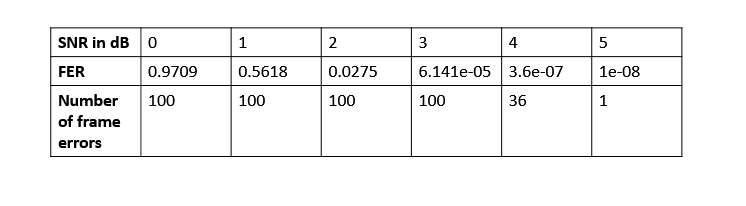
\includegraphics[width=0.8\textwidth]{FERTable.png}
	\caption{Data points from error plot simulation}
	\label{fig:ErrorTable}
\end{table}
\begin{figure}[!htb]
	\setlength\fwidth{0.95\textwidth}
	\setlength\fheight{0.4\textheight}
	\centering
	% This file was created by matlab2tikz.
%
%The latest updates can be retrieved from
%  http://www.mathworks.com/matlabcentral/fileexchange/22022-matlab2tikz-matlab2tikz
%where you can also make suggestions and rate matlab2tikz.
%
\definecolor{mycolor1}{rgb}{0.00000,0.44700,0.74100}%
%
\begin{tikzpicture}

\begin{axis}[%
width=0.951\fwidth,
height=\fheight,
at={(0\fwidth,0\fheight)},
scale only axis,
xmin=0,
xmax=6,
ymode=log,
ymin=1e-14,
ymax=1,
yminorticks=true,
axis background/.style={fill=white},
xmajorgrids,
ymajorgrids,
yminorgrids,
legend style={legend cell align=left, align=left, draw=white!15!black}
]
\addplot [color=mycolor1]
  table[row sep=crcr]{%
0	0.970873786407765\\
0.207089034514839	0.886158625566635\\
0.396468066078011	0.808688202487994\\
0.569679094946515	0.737831721822905\\
0.72813012135502	0.673013204420059\\
0.873108145518025	0.613706169336469\\
1.00127616687936	0.561115893572658\\
1.09610418268403	0.51044904154491\\
1.18304919717487	0.463994097334841\\
1.2628092104682	0.421378117690295\\
1.3360212226702	0.382260751820979\\
1.40326723387787	0.346331035582549\\
1.46507624417937	0.313306322871293\\
1.52193025365504	0.282929079808215\\
1.57426426237738	0.254966884739035\\
1.62247227041204	0.229209222418269\\
1.66690727781788	0.205467484009224\\
1.70788728464788	0.183571761268081\\
1.74569329094888	0.163371915149203\\
1.78057429676238	0.144734904291862\\
1.81274730212455	0.127544785020248\\
1.84240030706672	0.111701108435497\\
1.86969531161589	0.0971173175077392\\
1.89476831579472	0.0837207470760979\\
1.91773431962239	0.0714499523354174\\
1.93868832311472	0.060254174533614\\
1.95770832628472	0.0500917380637132\\
1.97485532914255	0.0409300504638505\\
1.99018033169672	0.0327418622986965\\
2.00276133379356	0.0274194345219116\\
2.09336934889489	0.0249337142898253\\
2.17646736274456	0.0226540217698943\\
2.25272137545356	0.0205620860624786\\
2.32273838712307	0.0186412548611499\\
2.38707339784557	0.0168763024162082\\
2.4462294077049	0.0152534295346823\\
2.50066341677724	0.0137600989776301\\
2.55078942513157	0.0123849531587889\\
2.59697943282991	0.0111177867107924\\
2.63956743992791	0.00994943675003731\\
2.67885144647524	0.00887172800911728\\
2.71509645251608	0.00787739053547292\\
2.74853345808891	0.006960087125175\\
2.77936446322741	0.0061142761540085\\
2.80776346796058	0.00533518414368909\\
2.83387847231308	0.00461875089429681\\
2.85783547630591	0.00396151974914304\\
2.87973647995608	0.00336069246233697\\
2.89966848327808	0.00281388229473649\\
2.91770048628342	0.00231919631529779\\
2.93388648898108	0.00187515309972576\\
2.94827249137875	0.00148049069399123\\
2.96089249348208	0.00113427634946393\\
2.97177549529592	0.000835714486429805\\
2.98094549682425	0.000584146694091027\\
2.98842449807075	0.000378969429216247\\
2.99423549903925	0.000219551714790884\\
2.99840949973492	0.000105043103534383\\
3.00218250036375	6.12764303565223e-05\\
3.09314251552375	5.57233513308062e-05\\
3.17656152942692	5.06306479529896e-05\\
3.25310754218459	4.5957539035856e-05\\
3.32339155389859	4.16667232240329e-05\\
3.38796956466159	3.77242568946278e-05\\
3.44734757455793	3.40992489088213e-05\\
3.50198358366393	3.07637385125039e-05\\
3.55229359204893	2.76923290381879e-05\\
3.59865159977527	2.48621879050069e-05\\
3.64139360689894	2.22528024199898e-05\\
3.6808206134701	1.98457966290168e-05\\
3.71719661953277	1.76250534161821e-05\\
3.75075462512577	1.55763482057052e-05\\
3.78169863028311	1.3687226862568e-05\\
3.81020263503377	1.19470667421963e-05\\
3.83641763940294	1.03466493426894e-05\\
3.86046864341144	8.87834345386468e-06\\
3.88246064707677	7.53573885916866e-06\\
3.90247865041311	6.31364633567718e-06\\
3.92059365343228	5.2077313560065e-06\\
3.93686165614361	4.21457513799476e-06\\
3.95132665855444	3.33149149565766e-06\\
3.96402466067078	2.55628264046258e-06\\
3.97498466249744	1.88717813164721e-06\\
3.98423066403844	1.32271277685641e-06\\
3.99178466529744	8.61543483098054e-07\\
3.99766966627828	5.02266107698561e-07\\
4.00213566702261	3.59252516542086e-07\\
4.09498568249761	3.26755011125835e-07\\
4.18012769668795	2.96955306159217e-07\\
4.25824370970729	2.6961470160245e-07\\
4.32995872165979	2.44514447419074e-07\\
4.39584073264012	2.21455743575957e-07\\
4.45640674273446	2.0025764004294e-07\\
4.51212575202096	1.80755986792665e-07\\
4.56342476057079	1.62801333800222e-07\\
4.6106867684478	1.46259631043272e-07\\
4.65425677570946	1.31010128501688e-07\\
4.6944437824073	1.16944676157446e-07\\
4.73151978858663	1.03968073994679e-07\\
4.76572579428763	9.19959719993285e-08\\
4.7972717995453	8.09548701591452e-08\\
4.8263388043898	7.07814184635697e-08\\
4.8530838088473	6.14206669034443e-08\\
4.87763681293947	5.28271154711861e-08\\
4.90010781668464	4.49622641603774e-08\\
4.9205868200978	3.77946129657689e-08\\
4.93914682319114	3.12986118831018e-08\\
4.95584782597464	2.54532609088769e-08\\
4.97073682845614	2.02421100403517e-08\\
4.98385083064181	1.56522092753681e-08\\
4.99521983253664	1.16730586121765e-08\\
5.00215983369331	9.97840166306694e-09\\
5.09263084877181	9.07369151228193e-09\\
5.17560486260081	8.24395137399188e-09\\
5.25174587529098	7.48254124709022e-09\\
5.32166088694348	6.7833911305652e-09\\
5.38590189765032	6.14098102349683e-09\\
5.44497290749548	5.55027092504515e-09\\
5.49932891655482	5.00671083445181e-09\\
5.54938292489715	4.50617075102846e-09\\
5.59550793258466	4.04492067415345e-09\\
5.63803593967266	3.61964060327344e-09\\
5.67726594621099	3.2273405378901e-09\\
5.71345995224333	2.86540047756675e-09\\
5.74685095780849	2.53149042191506e-09\\
5.77763896293983	2.22361037060173e-09\\
5.80599696766616	1.94003032333839e-09\\
5.83207397201233	1.67926027987671e-09\\
5.855993975999	1.44006024001004e-09\\
5.8778609796435	1.22139020356504e-09\\
5.89775998296	1.02240017040002e-09\\
5.91575898595983	8.42410140401685e-10\\
5.93191398865233	6.80860113476686e-10\\
5.94626899104483	5.37310089551681e-10\\
5.95885899314317	4.11410068568348e-10\\
5.969711994952	3.02880050480008e-10\\
5.97885199647533	2.1148003524667e-10\\
5.986301997717	1.36980022830002e-10\\
5.99208399868067	7.9160013193338e-11\\
5.99622999937167	3.77000062833321e-11\\
5.99878899979817	1.21100020183373e-11\\
5.99988099998017	1.19000019833671e-12\\
5.99999899999983	1.00000016622914e-14\\
};
\addlegendentry{data1}

\end{axis}
\end{tikzpicture}%
	\caption{Plot of error floor calculation}
	\label{fig:ErrorFloor}
\end{figure}
As mentioned before a minimum number of frame errors are needed to confirm a \gls{FER}. While 36 frame errors are not the optimal number of errors it is still enough to validate an error floor of $10^{-6}$.
Seen in \fig{fig:ErrorFloor} the \gls{FER} decreases ever so slowly for higher \gls{SNR}. The break in the rapid decrease of \gls{FER} indicates the start of the error floor, also called "watefall" curves\cite{Richardson}. 
 






\clearpage
